\documentclass{beamer}
% Setup appearance:
\usetheme{Berkeley} 

\usepackage{color} % It may be necessary to set PCTeX or whatever program you are using to output a .pdf instead of a .dvi file in order to see color on your screen.
\usepackage{graphicx} 

\usepackage[spanish]{babel}
\usepackage[latin1]{inputenc}
\usepackage{amsmath}
\usepackage{mathtools}
\usepackage{calrsfs}
\usepackage{cases}
\usepackage{hyperref}

\usepackage{tikz}
\usetikzlibrary{arrows}
\tikzstyle{block}=[draw opacity=0.7,line width=1.4cm]


% Author, Title, etc.

\title[] 
{%
  Introducci�n al CIAA Firmware\\ Ejercitaci�n %
}
	
\author[]
{
   Ing. Gustavo Muro - Bioing.~Juan~Manuel Reta~\
}

%\insertshortdate
\date[2015]
{4ta Escuela de Sistemas Embebidos}


% The main document

\begin{document}

\begin{frame}
% \begin{center}

%\end{center}
  \titlepage
\begin{center}
  
	
\includegraphics[height=1cm]{Imagenes/logo_ruse}
\hspace{1cm}
	
\includegraphics[height=1cm]{Imagenes/acse}
\end{center}

\end{frame}

\section{Tool Chain}

\begin{frame}{Ejemplo de Tool Chain}	

\begin{figure}
		\centering
		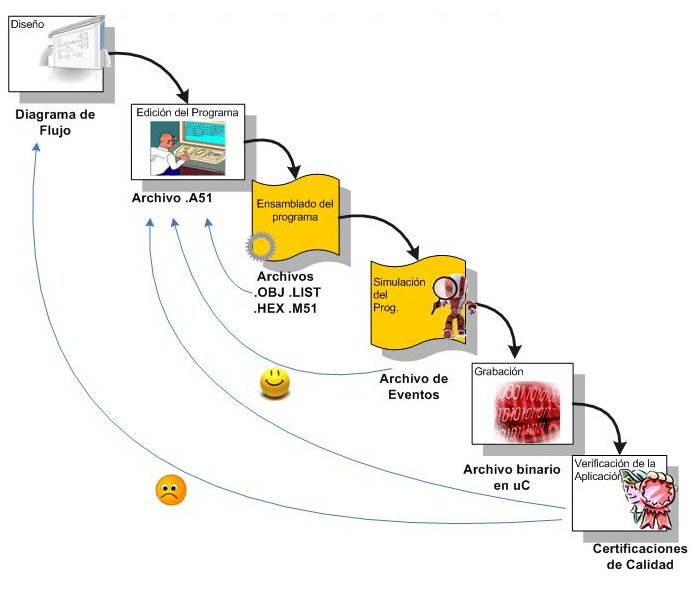
\includegraphics[height=7.5cm]{Imagenes/toolchain}
		\label{fig:toolchain}
\end{figure}
 
\end{frame}


\begin{frame}{Tool Chain CIAA y EDU-CIAA}	

Para desarrollar aplicaciones con al EDU-CIAA se trabajar con las siguientes herramientas:

\begin{itemize}
\item Compilador ARM-GCC 
\item Procesador PHP
\item OpenOCD
\end{itemize}
\vspace{1cm}
\begin{center}

\includegraphics[height=1cm]{Imagenes/gnu_arm}
\hspace{1 cm}

\includegraphics[height=1cm]{Imagenes/php}
\end{center}

\end{frame}


\begin{frame}{Target}

El entorno empleado est� basado en Eclipse \textbf{Eclipse Kepler o Luna}

\begin{center}

\includegraphics[height=3cm]{Imagenes/eclipse}
\end{center}

\end{frame}


\begin{frame}{RTOS - FreeOSEK}

Una gran parte del desarrollo del firmware de la CIAA se basa en la implementaci�n de un Sistema Operativo de Tiempo Real (RTOS) - FreeOSEK.\\

Para el proceso de compilaci�n del RTOS-OSEK, se emplea PHP (lenguaje interpretado de alto nivel).

\vspace{1cm}
\begin{center}

\includegraphics[height=1cm]{Imagenes/php}
\end{center}

\end{frame}


\section{Conceptos}
\subsection{Testing}

\begin{frame}{Testing}
\vspace{0.5 cm}
\begin{columns}
\column{.65\textwidth}
El testing es una actividad desarrollada para \textbf{evaluar la calidad} del producto, y para mejorarlo al \textbf{identificar defectos} y problemas.\\
El testing de software consiste en la \textbf{verificaci�n din�mica del comportamiento} de un programa sobre un \textbf{conjunto finito de casos de prueba}.
\column{.25\textwidth}
\begin{flushright}

\includegraphics[height=2.5cm]{Imagenes/testing3}
\end{flushright}
\end{columns}

\begin{figure}
		\centering
		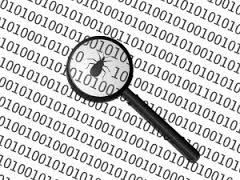
\includegraphics[height=3cm]{Imagenes/testing2}
		\label{fig:testing}
\end{figure}
			
\end{frame}

\begin{frame}{Testing: Tipos de Testeos}

	\begin{figure}
			\centering
			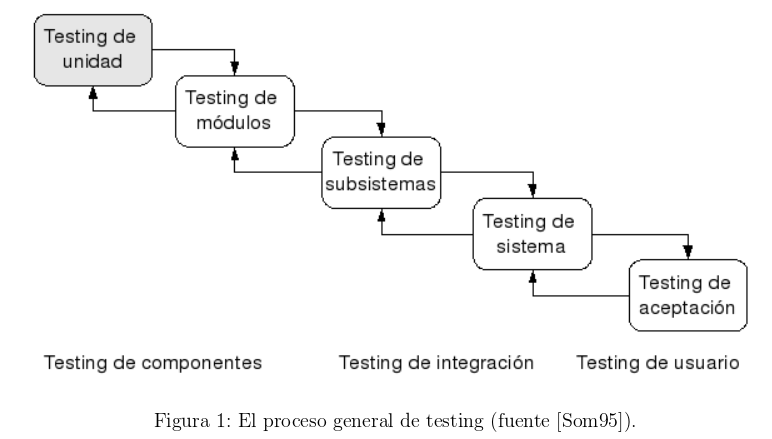
\includegraphics[height=6cm]{Imagenes/testing}
			\label{fig:testing}
			\end{figure}
\end{frame}

\begin{frame}{Tool Chain}	
\begin{center}
{\Large �En cu�l etapa se dise�an las funciones de testeo? \\
�En que etapa se se realiza el testing?}
\end{center}
\begin{figure}
		\centering
		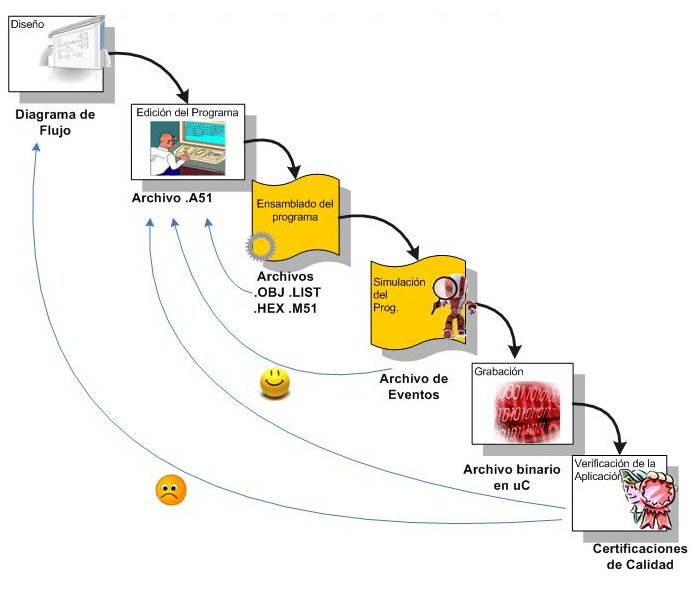
\includegraphics[height=6cm]{Imagenes/toolchain}
		\label{fig:toolchain}
\end{figure}
 
\end{frame}

\subsection{Versionado}

\begin{frame}{Respositorios}

\begin{block}{Concepto}
Un repositorio es un sitio en el cual se almacena almacena y mantiene informaci�n digital, habitualmente bases de datos o archivos.
\end{block}

\begin{center}
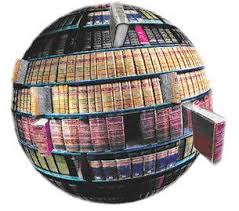
\includegraphics[height=3cm]{Imagenes/repo1}
\end{center}

\end{frame}

\begin{frame}{Gestores de Respositorios}

\begin{itemize}
\item SVN
\item GIT
\item Mercurial
\end{itemize}

\begin{columns}
\column{.4\textwidth}
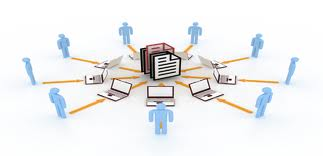
\includegraphics[height=3cm]{Imagenes/repo_centralizado}
\column{.5\textwidth}
\begin{flushright}
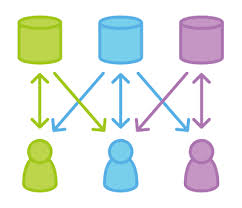
\includegraphics[height=3cm]{Imagenes/repositorio}
\end{flushright}
\end{columns}

\end{frame}

\begin{frame}{Conceptos}

\begin{center}
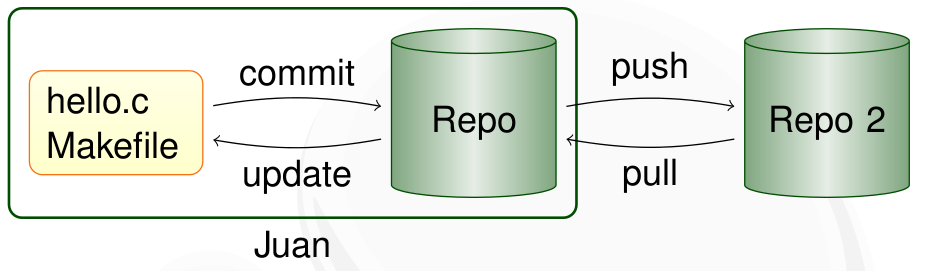
\includegraphics[height=2cm]{Imagenes/repo_modo_trabajo}\\
%\textbf{Proceso de Impresi�n 3D}
\end{center}

\begin{itemize}
\item \textbf{Directorio de trabajo:} Es un directorio donde est�n los archivos que queremos administrar.
\item \textbf{Changeset:} Conjunto de cambios en los archivos entre una revisi�n y la siguiente.
\item \textbf{Repositorio:} Guarda el historial de nuestro trabajo (almacena los changesets).
\end{itemize}

\end{frame}

\begin{frame}{Modo de Trabajo}
\begin{center}
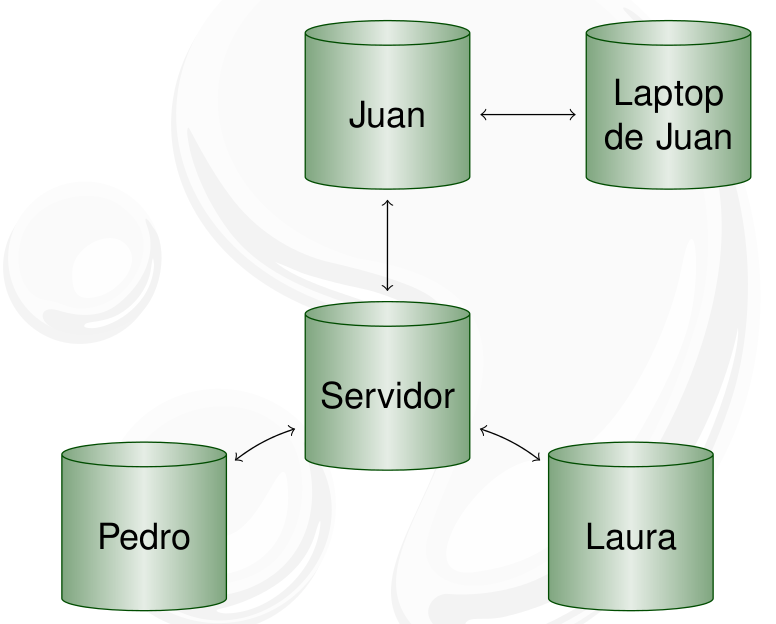
\includegraphics[height=5cm]{Imagenes/repo_changeset13}%\textbf{Simulaci�n Num�rica}
\end{center}

\end{frame}

\begin{frame}{Modo de Trabajo}
\begin{center}
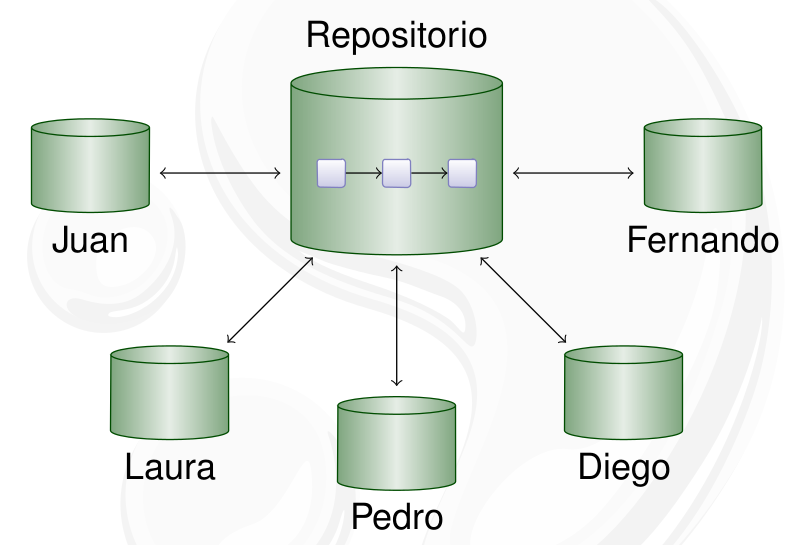
\includegraphics[height=5cm]{Imagenes/repo_changeset14}%\textbf{Simulaci�n Num�rica}
\end{center}

\end{frame}

\begin{frame}{Branches}

Se trata de un concepto clave:\\
Permite trabajar en l�neas de desarrollo paralelas, que posteriormente pueden ser empeladas para generar un \textit{release}.\\

\begin{center}
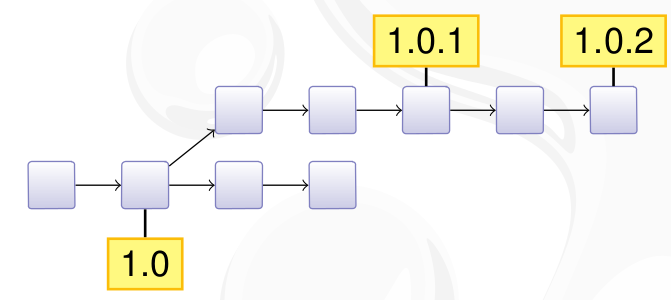
\includegraphics[height=3cm]{Imagenes/repo_branch1}
\end{center}
\end{frame}

\begin{frame}{Merge}

Es lo opuesto al branch:\\
Se emplea para combinar lineas de trabajo paralelas o secillamente diferentes. Tambi�n es empleado para traer arreglos realizados en otros branches.


\begin{center}
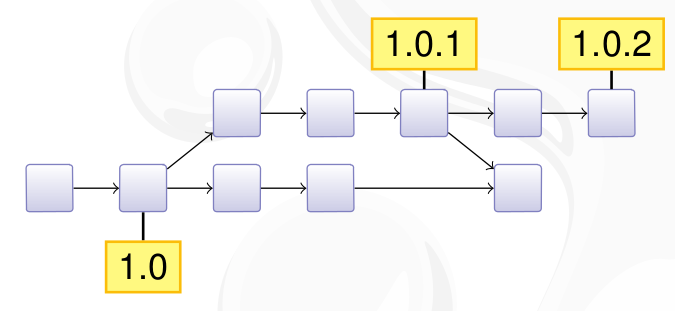
\includegraphics[height=3cm]{Imagenes/repo_merge1}
\end{center}
\end{frame}

\begin{frame}{Herramienta Libre: GitHub}

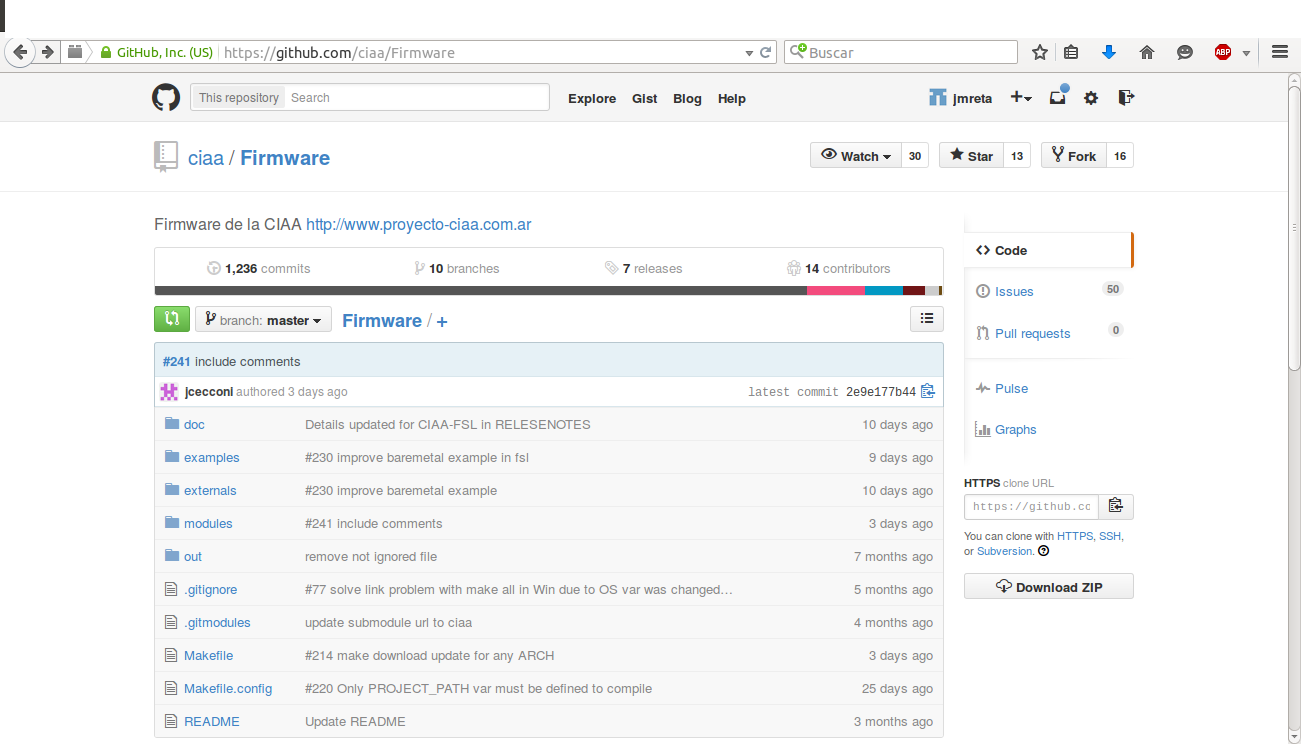
\includegraphics[height=6.5cm]{Imagenes/github}
\end{frame}



\section{Ejercitaci�n}

\begin{frame}{Ejercitaci�n}

\begin{center}

\includegraphics[height=3cm]{Imagenes/ejercicios}
\end{center}

\end{frame}

\subsection{Practica 1}
\begin{frame}{Ejercitaci�n}

\begin{block}{Pr�ctica 1}
Dise�e e implemente un sistema que haga titilar un led con un
periodo comprendido entre 100 y 1000 ms. El sistema debe
permitir seleccionar uno de entre 6 leds disponibles y el valor
del periodo de parpadeo.\\

\end{block}

\begin{center}
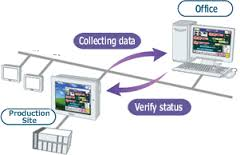
\includegraphics[height=3 cm]{Imagenes/remote_access}
\end{center}

\end{frame}

\begin{frame}{Ejercitaci�n}

\underline{Interfaz Local:}

\begin{itemize}
\item Tec 1: Selecciona LED a la Izquierda para parpadeo.
\item Tec 2: Selecciona LED a la Derecha para parpadeo
\item Tec 3: Incrementa el periodo de parpadeo en 10 ms.
\item Tec 4: Decrementa el periodo de parpadeo en 10 ms.
\end{itemize}
\hspace{0.3 cm}
\begin{columns}			
\column{.45\textwidth}

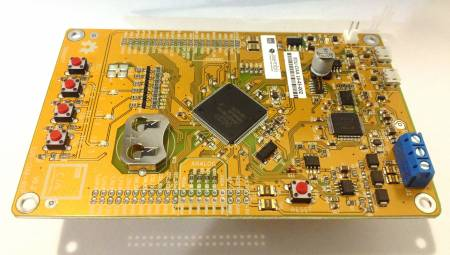
\includegraphics[height=3cm]{Imagenes/EDU_CIAA_placa}

\column{.45\textwidth}
\begin{center}

\href{https://github.com/gmuro/ejercicioFinal}
         {
\includegraphics[height=1cm]{Imagenes/github1}}\\
         
Descargue la plantilla disponible en GitHub\\ (click sobre el icono)     
\end{center}
\end{columns}

\end{frame}

\begin{frame}{Ejercitaci�n}

\begin{itemize}
\item Se deber� implementar la funci�n disponible  \href{https://github.com/gmuro/ejercicioFinal/blob/master/src/modbusSlave.c#L202}{\underline{\textbf{\textcolor[rgb]{0,0.5,0.5}{aqu�}}}}.La misma ser� ejecutada autom�ticamente por el protocolo de comunicaci�n modbus, cada vez que el Master oprima una tecla.\footnote{El dato recibido conserva el mismo formato que el accedido por el teclado local.}\\
\item El Master necesitar� conocer el estado de los leds, para est� ejecutar� la funci�n disponible \href{https://github.com/gmuro/ejercicioFinal/blob/master/src/modbusSlave.c#L142}{aqu�}, que devolver� el estado de los leds en ese momento.
\item  Ser� responsabilidad del programador, llamar a las funciones \href{https://github.com/gmuro/ejercicioFinal/blob/master/src/modbusSlave.c#L281}{\underline{\textbf{\textcolor[rgb]{0,0.5,0.5}{modbusSlave}}}} y 
\href{https://github.com/gmuro/ejercicioFinal/blob/master/src/teclado.c#L99}{\underline{\textbf{\textcolor[rgb]{0,0.5,0.5}{teclado}}}} con un per�odo de 10 milisegundos.
\item Considerar que el parpadero de los leds, debe tener el menor \textit{jitter} posible.
\end{itemize}


\end{frame}


\begin{frame}{}


\begin{center}

\includegraphics[height=4cm]{Imagenes/continuara}
\end{center}

\end{frame}

\end{document}
